%**********************************************************
\section{Local System}
%**********************************************************
\subsection{Task Overview}
One can define and describe briefly how the local system is implemented, making use of threads and processes. As one can see in figure \ref{fig:task_overview}, this system is composed by two processes: the main process and a daemon, used to read the sensors \textit{LDR} and \textit{LampFailureDetector}, \textit{dSensors}. As the \textit{PIR} sensor can be read through the use of an ISR, this sensor stays in the main process. The communication between the daemon and the main process is done via message queue.

\begin{figure}[H]
	\centering
	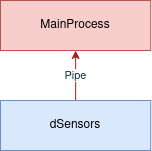
\includegraphics[width=.3\textwidth]{09sw_specification/task_overview}
	\caption{Inter-process Communication between Main Process and Daemon.}
	\label{fig:task_overview}
\end{figure}

\clearpage
One can list the tasks that compose the main process:
\begin{itemize}
	\item \textbf{tCamera:} acquire a camera frame; processes image and search for parking spots; verify the parking spot availability;
%	\item \textbf{tLampControl:} initializes PWM interface; controls the PWM applied to the lamp;
	\item \textbf{tLoraSend:} sends a message to the gateway, using the LoRa module;
	\item \textbf{tLoraRecv:} receives a message from the gateway, using the LoRa module;
	\item \textbf{tRecvSensor:} receives messages sent by the daemon, via message queue, regarding sensors information.
\end{itemize}

%**********************************************************
\subsection{Task Priority}

%**********************************************************
\subsection{Task Synchronization}
Real-time tasks share resources and services, and as such, should be prepared to await for the availability of these resources and services, like logical resources (buffers and data), physical resources, services like directory services, etc. In order to have coordinate access to shared resources and avoid race conditions, the kernel has resources that provide synchronization tools. 

\myparagraph{Condition Variables}

A condition variable is a task synchronization tool that can be used to block (wait) one or more threads, suspending its execution. The blocked threads are awakened when the condition variable is notified. The condition variables used are listed below.

\begin{itemize}
	\item \textbf{condCameraAcquire:} used to notify \textit{tCamera} that a camera sample period has elapsed;
	
%	\item \textbf{condNewPWM:} used to notify \textit{tLampControl} that a new PWM value for the lamp was defined;
	
	\item \textbf{condSend:} used to notify \textit{tLoraSend} that a new message is ready to be sent;
	
	
\end{itemize}

\myparagraph{Mutexes}

A mutex is a locking mechanism that provides mutual exclusion, supporting ownership and other protocols. A mutex is initially created in the unlocked state in which it can be acquired by a task. After being acquired, the mutex moves to the locked state. When the task releases the mutex, it returns to the unlocked state. The mutexes used are listed bellow.

\begin{itemize}
	\item \textbf{mutCamera:} mutex associated with the condition variable \textit{condCameraAcquire} to acquire a camera frame;
		
	\item \textbf{mutSend:} protects the message to be sent in \textit{tLoraSend}, which can be defined in multiple places;
	
	\item \textbf{mutComms:} protects LoRa communication, since it is half-duplex, so one can send or receive at a time; Used in \textit{tLoraSend} and \textit{tLoraRecv};
	
	\item \textbf{mutChangePWM:} protects the modification of PWM when defining a new PWM value for the lamp;
	
	
\end{itemize}

%\myparagraph{Semaphores}

\subsection{Task Communication}
%\myparagraph{Pipes}
%
%Pipe is an inter-process communication tool, that establishes a connection between two processes, such that the standard output from one process becomes the standard input of the other process. Pipe is one-way communication, i.e, we can use a pipe such that one process write to the pipe and the other process reads from the pipe. If a process tries to read before something is written to the pipe, the process is suspended until something is written.
%
%As previously stated, it's used a pipe to communicate between the \textit{dSensors} to the main process. In this way, the main process can know if something was detected by the sensors and provide a response to that.

\myparagraph{Message Queue}

A message queue is a linked list of messages stored within the kernel and identified by a message queue identifier. A message queue will be used to communicate between the main process and the \textit{dSensors}. In that way, the main process is agnostic to the cyclic reading necessary for the sensors \textit{LDR} and \textit{LampFailureDetector}, and is only informed when necessary, thorough the message queue.

%**********************************************************
\subsection{Class Diagrams}
\myparagraph{Class Camera}

In figure \ref{fig:classcamera} is shown the Camera class diagram, that defines a camera object.  For this project the camera is used to detect available parking spots in the lamppost vicinity, so this class defines the functions used to capture (\textit{captureFrame()}) and process (\textit{processFrame}) a camera frame. After the creation of the object, using the constructor \textit{Camera()}, the thread \textit{tCamera()} is executed every time the condition variable \textit{condCameraAcquire} is signaled, that happens every 2 minutes.

%This class defines all the functions that implicate the use of the camera device.

\begin{figure}[H]
	\centering
	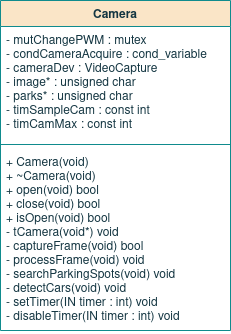
\includegraphics[width=.5\textwidth]{09sw_specification/classcamera}
	\caption{Class Diagram: Camera.}
	\label{fig:classcamera}
\end{figure}

\myparagraph{Class Lamp}

In figure \ref{fig:classlamp} is shown the Lamp class diagram, which defines a Lamp object. After creating the object, using the constructor \textit{Lamp()}, one can interact with it by changing the brightness, through the method \textit{setBrightness(lux)}, where \textit{lux} is a value from 0, lamp OFF, to 100, lamp at maximum brightness. Internally, this class uses a mutex, \textit{mutChangePWM} to protect the PWM value when using \textit{setBrightness} method. 

\begin{figure}[H]
	\centering
	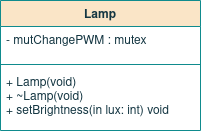
\includegraphics[width=.5\textwidth]{09sw_specification/classlamp}
	\caption{Class Diagram: Lamp.}
	\label{fig:classlamp}
\end{figure}

\myparagraph{Class Communications}

In figure \ref{fig:classcomm} is shown the Communications class diagram. This class defines an object Communication capable of establishing a LoRa communication with the gateway, through the use of the constructor \textit{Communication()}, and send messages through the use of \textit{Send(msg)}. It's used a vector of messages \textit{queued\_msgs} to store the message that's in the waiting list to be sent, in order to avoid the loss of a communication. To exchange messages are used two threads, \textit{tLoraSend} to send, and \textit{tLoraRecv} to receive, which makes use of task synchronization tools to ensure that sending and receiving don't occur at the same time, since the LoRa module in use is Half-Duplex.

\begin{figure}[H]
	\centering
	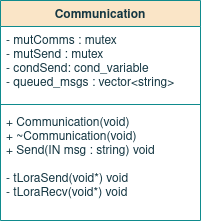
\includegraphics[width=.5\textwidth]{09sw_specification/classcomms}
	\caption{Class Diagram: Communications.}
	\label{fig:classcomm}
\end{figure}

%**********************************************************
\subsection{Flowcharts}
%\clearpage
\myparagraph{tCamera}

The task tCamera is responsible for acquire a frame from the Raspberry Pi Camera and to process it. It must analyze the returned frame, in order to detect empty parking spots. This thread uses the mutex \textit{mutCamera} to protect the condition variable \textit{condCameraAcquire}, that synchronizes the camera frame acquisition with the timer that defines the camera frame acquisition period, \textit{timSampleCam}.

Firstly, this thread initializes the camera device, sets the timer \textit{timSampleCam}, locks the mutex \textit{mutCamera} and goes to sleep mode, waiting for the conditon variable \textit{condCameraAcquire} to be signaled. This happens when a \textit{timSampleCam} period has elapsed and the thread wakes up. Now, one can capture a camera frame in order to process it, unlocking the mutex \textit{mutCamera}. A timer, \textit{timCamMax}, is setted to report the error if the image is taking too much time to being processed.

In the image processing part of the thread, if there aren't parking spots coordinates stored, then it is necessary to search for parking spots. After that, one can detect cars using the pre-trained model and the function \textit{detectCars} that detects cars in the image. If the coordinates of a detected car matches the coordinates of the parking spot, then one can assume that the parking spot is occupied. If the parking spot status has changed, then it is necessary to send this to the remote system, using the LoRa communication module.

\myparagraph{tRecvSensors}

This task, presented in figure \ref{fig:flow_trecv_sensors}, is responsible for receiving messages sent by the sensors daemon, through a message queue.

When the message queue is not empty, this task reads a message from the message queue and parses it, in order to find out which sensor was triggered and what action this system should take. For that, a list of commands may be defined:
\begin{itemize}
%	\item Lamp Max: the lamp brightness must be at its maximum (PWM=100);
	\item Lamp Min: the lamp must be at minimum bright level (PWM = \textit{MIN\_BRIGHT\_PWM});
	\item Lamp OFF: the lamp must be OFF (PWM=0);
	\item Lamp Fail: the lamp must be OFF, since there was a failure detected on the lamp.
\end{itemize}

\begin{figure}[H]
	\centering			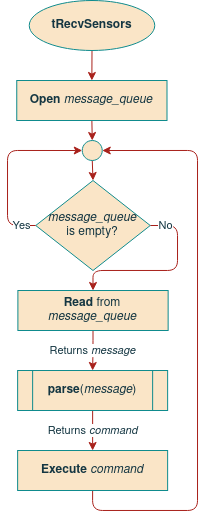
\includegraphics[width=.4\textwidth]{09sw_specification/trecvsensors}
	\caption{Main Process Flowchart: tRecvSensors.}
	\label{fig:flow_trecv_sensors}
\end{figure}

%**********************************************************
\clearpage
\myparagraph{Class Lamp Constructor and Destroyer}

This functions, presented in figure \ref{fig:flow_lampconstruct}, are responsible for initializing and destroying a Lamp object. First, in the constructor, which is the left side function, the PWM peripheral is initialized, then the mutex that is used to protect the change of PWM is also initialized. On the destroyer side, the opposite is done, by the terminating the PWM generation.

\begin{figure}[H]
	\centering	
	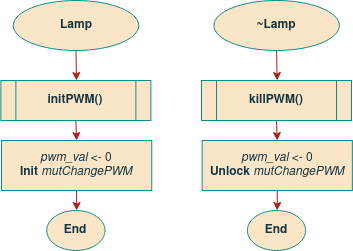
\includegraphics[width=.7\textwidth]{09sw_specification/lampconstruct}
	\caption{Class Lamp Flowchart: Constructor and Destroyer.}
	\label{fig:flow_lampconstruct}
\end{figure}

\myparagraph{setBrightness}

This function, presented in figure \ref{fig:flow_setbrightness}, is responsible for changing the PWM associated with the lamp, which is directly related to its brightness. Through \textit{setPWM(lux)} one can change the current lamp PWM to \textit{lux} value, being this an integer between 0 to 100. When the PWM is maximum, a timer is started that defines how much time the lamp is ON, \textit{LAMP\_ON\_TIMEOUT} in seconds, if there isn't another call of this function.

\begin{figure}[H]
	\centering	
	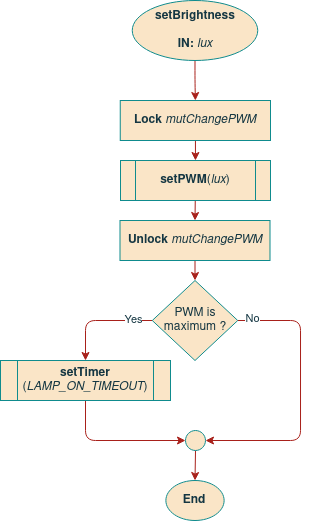
\includegraphics[width=.6\textwidth]{09sw_specification/lampsetbrightness}
	\caption{Class Lamp Flowchart: setBrightness.}
	\label{fig:flow_setbrightness}
\end{figure}


%**********************************************************
\clearpage
\myparagraph{Class Communication Constructor and Destroyer}

This functions, presented in figure \ref{fig:flow_commconstruct}, are responsible for initializing and destroying a Communication object. On the left side, the constructor, starts by initializing the LoRa communication, defining the frequency in which the device choosen previously operates, which is 433~MHz. Then the messages vector is cleared, the mutexes are initialized and the two threads responsible for the exchange of messages between the local system and the gateway are created. In the destroyer side, one has the opposite, where the LoRa communication is disabled and the threads are terminated.

\begin{figure}[H]
	\centering			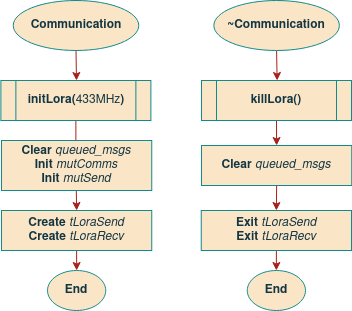
\includegraphics[width=.7\textwidth]{09sw_specification/commsconstruct}
	\caption{Class Communication Flowchart: Constructor and Destroyer.}
	\label{fig:flow_commconstruct}
\end{figure}

\myparagraph{tLoraSend}

This task is responsible for sending queued messages to the gateway, using LoRa communication. A conditional variable is used to wake this thread when there is a new message available to be sent.

When the vector \textit{queued\_msgs} is empty, then the task goes to sleep, waiting for the condition variable \textit{condSend} to notify this task. This happens when a new message is inserted into the messages vector, using \textit{Send(msg)} function, that will be later presented. After this, the mutex \textit{mutComms} is used to protect the communication, which due to the selected LoRa module is half-duplex, meaning that at a given moment, the device can be receiving or sending, not at the same time. Then, a message is popped from the messages vector, and sent to the gateway using the function \textit{LoraSend}. This continues to happen until the \textit{queued\_msgs} vector gets empty.

The flowchart for this task is presented in figure \ref{fig:flow_tlorasend}

\begin{figure}[H]
	\centering		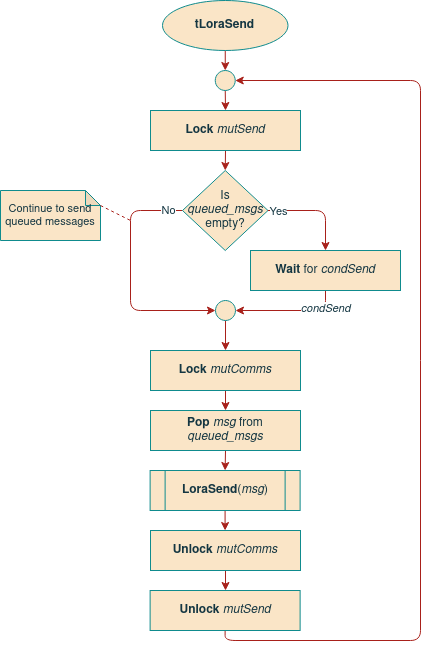
\includegraphics[width=.85\textwidth]{09sw_specification/commstlorasend}
	\caption{Class Communication Flowchart: tLoraSend.}
	\label{fig:flow_tlorasend}
\end{figure}


\myparagraph{tLoraRecv}

This task is responsible for receiving messages from the gateway, using LoRa communication.

When a message is received, using \textit{LoraReceive}, this is parsed and later, the respective command will be executed.

The flowchart for this task is presented in figure \ref{fig:flow_tlorarecv}

\begin{figure}[H]
	\centering		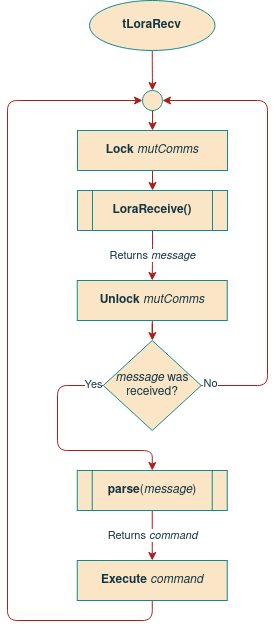
\includegraphics[width=.55\textwidth]{09sw_specification/commstlorarecv}
	\caption{Class Communication Flowchart: tLoraRecv.}
	\label{fig:flow_tlorarecv}
\end{figure}

\myparagraph{Send}

This function, presented in figure \ref{fig:flow_send}, is responsible for adding a new message, \textit{msg}, to the \textit{queued\_msgs} vector, and signal the condition variable \textit{condSend}, for the task \textit{tLoraSend} to send the message.

\begin{figure}[H]
	\centering	
	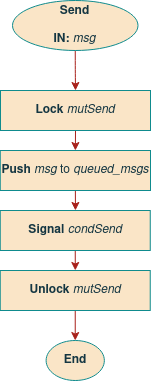
\includegraphics[width=.3\textwidth]{09sw_specification/commssend}
	\caption{Class Communication Flowchart: Send.}
	\label{fig:flow_send}
\end{figure}


% FLOWCHARTS SENSORS

\myparagraph{PirIsr}
The PIR sensor uses the GPIO of the Raspberry Pi in order to inform the system if there's movement in the surrounding area. In the afirmative case, it puts the high digital value on its output, and this can be used to generate an interrupt service routine, triggered on the rising edge of the output signal of the sensor. When this routine is executed, it locks the mutex \textit{mutChangePWM} and assign the \textit{PWM\_val} its maximum value, 100 \%, unlocking the mutex. Now, one needs to send the PWM value to the remote system through the LoRa communications, in order to be updated in the remote system. In the figure \ref{fig:pir_isr}, is represented the flowchart of the PirIsr function.

\begin{figure}[H]
	\centering
	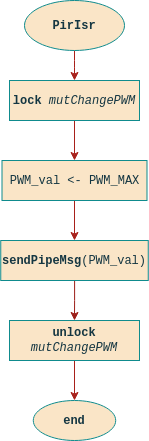
\includegraphics[width=.2\textwidth]{09sw_specification/pir_isr}
	\caption{PirIsr flowchart.}
	\label{fig:pir_isr}
\end{figure}

\myparagraph{LdrIsr}
The ambient light sensor, LDR, is used to determine when is time to turn on the lights, that is, when is night time and interfaces with the Raspberry Pi through I2C protocol communication. As the sun set or the sun rise is a relatively long time process, there's no need to keep checking the sensor output value all the time, so one can define a period to get the sensor value, \textit{LDR\_TIM}, that can be 10 minutes. In figure \ref{fig:ldr_isr} is shown the LDR sensor interrupt service routine, triggered by the timer overflow. When the timer period elapses, the illuminance value is calculated by the sensor. If this value is lower than the threshold value defined as good luminosity illuminance, GOOD\_LIGHT\_LUX, then the auxiliary variable, \textit{lightCon} is setted to high. In the next step, if the \textit{oldLightCon} variable (stores the last ambient light condition) is not equal to the auxiliary variable, then it is needed to change the \textit{oldLightCon} variable and send message to the process that controls the lamp PWM, through message queue. 

\begin{figure}[H]
	\centering
	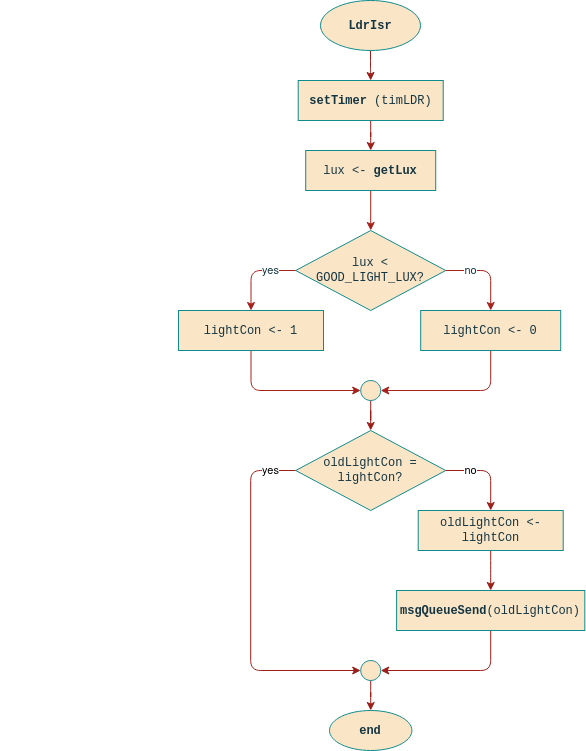
\includegraphics[width=.4\textwidth]{09sw_specification/ldr_isr}
	\caption{LdrIsr flowchart.}
	\label{fig:ldr_isr}
\end{figure}

\myparagraph{FailureDetectIsr}
In figure \ref{fig:fail_isr} is represented the FailureDetectIsr flowchart. Similarly to the PIR sensor, this routine is triggered on the rising edge of the output signal of the sensor. When the Failure detector detects that the lamp is broken, it puts the high digital value in its output, triggering this function. In this routine, the PWM is setted to 0 \% and are sent two messages through message queue: one to inform the process, that controls the lamp, to change the PWM value in the channel; and the other to notify the remote system that the lamp is broken, in order to update this status on the database.

\begin{figure}[H]
	\centering
	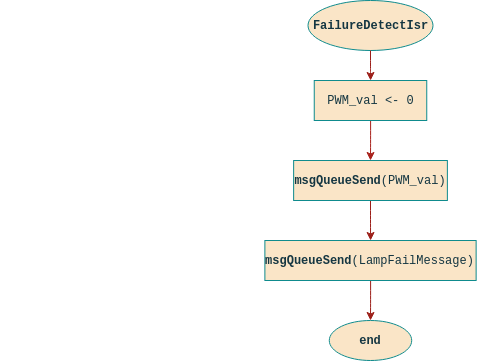
\includegraphics[width=.3\textwidth]{09sw_specification/fail_isr}
	\caption{FailureDetectIsr flowchart.}
	\label{fig:fail_isr}
\end{figure}

%**********************************************************
\subsection{Start-up Process}

%**********************************************************
\subsection{Shutdown Process}

%\myparagraph{tLampControl}
% uses: mutChangePWM; condNewPWM; pwm_val
% pwm_val is used in: PIR_sensor, CommandCb, LDR
% must define: MIN_BRIGHT_PWM; LAMP_ON_TIMEOUT
%This task is responsible for initializing and controlling the PWM peripheral used to control the lamp brightness. A mutex \textit{mutChangePWM} is used to protect the process of defining a new PWM value. 
%
%After initializing the PWM, this task goes to sleep, waiting for the condition variable \textit{condNewPWM} to notify this task. This happens when a new PWM value is defined into the variable \textit{pwm\_val}, in \textit{dReadSensors} or in a received command. Then, the lamp PWM is changed to the new value. 
%
%The lamp may have various levels of luminosity: for the lamp to be OFF, is applied PWM~=~0; for the lamp to be at a predefined minimum bright level, is applied PWM~=~\textit{MIN\_BRIGHT\_PWM}; for the lamp to be at maximum bright, this is, when the lamp must be ON, is applied PWM~=~100. So, since the lamp must stay ON a minimum amount of time out of a motion is detected or out of a request from the remote system to be ON, one needs to check if the new PWM is the maximum value. If so, that means that the lamp should continue with that PWM for a predefined time, defined by \textit{LAMP\_ON\_TIMEOUT}, in seconds.


%**********************************************************
\clearpage
\section{Gateway}
One can define the relationship between the tasks as follows, in figure \ref{fig:GwOverview}. The rule of the gateway is to receive LoRa messages and send the content in TCP-IP messages, or vice versa.

\begin{figure}[H]
	\centering
	\includegraphics[width=1\textwidth]{09sw_specification/Gateway/overview}
	\caption{Gateway Overview.}
	\label{fig:GwOverview}
\end{figure}

%**********************************************************
\subsection{Class Diagrams}
In figure \ref{fig:GwclassDiag} is represented the class diagram of gateway, \textit{CGateway}, which is the main class of the system, responsible for initializing the objects of each class listed below.

\begin{itemize}
	\item \textbf{CLoraComm:} manages the LoRa communications with the local systems, interfacing with the LoRa module; this class was already detailed previously;
	
	\item \textbf{CTCPclient:} manages the TCP-IP communication with the remote server;
\end{itemize}

\begin{figure}[H]
	\centering	\includegraphics[width=.68\textwidth]{09sw_specification/Gateway/cgateway/class}
	\caption{CGateway Class Diagram.}
	\label{fig:GwclassDiag}
\end{figure}

\myparagraph{Class CTCPclient}

In figure \ref{fig:TCPclientClass} is shown the CTCPclient class. This class defines a TCPclient capable of establishing a connection to a given remote server and to exchange messages to it, via TCP-IP. Like in the CLoraComm class, this class inherits from the class CCommunication.

\begin{figure}[H]
	\centering
	\includegraphics[width=.4\textwidth]{09sw_specification/Gateway/ctcpclient/class}
	\caption{Class Diagram: TCPclient.}
	\label{fig:TCPclientClass}
\end{figure}

%**********************************************************
\clearpage
\subsection{Task Overview}
One can define and describe briefly how the gateway is implemented, making use of threads and processes.

\begin{itemize}
	\item \textbf{tLoraRecv:} receives all messages from local systems, using LoRa communication;
	\item \textbf{tTCPRecv:} receives all messages from the remote server, using TCP-IP communication;	
	\item \textbf{CLoraComm::tSend:} sends all received messages from the remote server, in \textit{tTCPRecv}, to the local systems, using LoRa communication; 
	\item \textbf{CTCPclient::tSend:} sends all received messages from local systems, in \textit{tLoraRecv}, to the remote server, using TCP-IP communication;
\end{itemize}

%**********************************************************
\subsection{Task Priority}
The priority assignment diagram for the gateway is represented in figure \ref{fig:gwt_priority}.

\begin{figure}[H]
	\centering
	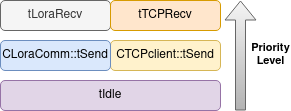
\includegraphics[width=0.6\textwidth]{09sw_specification/Gateway/priority}
	\caption{Gateway Priority Assignment Schematic.}
	\label{fig:gwt_priority}
\end{figure}

%**********************************************************
\subsection{Task Synchronization}

\myparagraph{Condition Variables}

The condition variables used in this system are listed below.

\begin{itemize}
	\item \textbf{CCommunication::condSend:} already detailed in the local system section; this condition variable is used indirectly by \textit{CTCPclient} and \textit{CLoraComm}.
\end{itemize}

\myparagraph{Mutexes}

The mutexes used in this system are listed bellow.

\begin{itemize}
	\item \textbf{CCommunication::mutComms} and \textbf{CCommunication::mutTxMsgs:} already detailed in the local system section; this mutexes are used indirectly by \textit{CTCPclient} and \textit{CLoraComm}.
\end{itemize}

%%**********************************************************
\subsection{Start-up Process}
In figure \ref{fig:bootGateway} is shown the start-up process for the gateway. When booting up, the gateway creates a CGateway object, initializing all needed members, and after that, runs until all the threads termination.

\begin{figure}[H]
	\centering		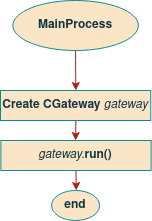
\includegraphics[width=.3\textwidth]{09sw_specification/Gateway/mainprocess}
	\caption{Start-Up Process: Gateway.}
	\label{fig:bootGateway}
\end{figure}

%**********************************************************
\clearpage
\subsection{Flowcharts}
%Each local system has a predefined ID, which may be presented in a physical label for an operator to use this information. When a local system is being installed, it will use it's predefined ID in all communications with the remote server until the operator registers the local system that's being installed, in the remote server. By doing this, the remote server assigns a new ID to the local system, which is then sent to the local system, for this to be used in further communications.

%*****************************
\myparagraph{CGateway Methods}

In figure \ref{fig:gwtCGatewayconstructor} is shown the \textit{CGateway} class constructor. With this, one can create a CTCPclient and a CLoraComm objects. After this the threads are created and both objects begin running their threads for receiving and sending messages.

\begin{figure}[H]
	\centering
	\includegraphics[width=.3\textwidth]{09sw_specification/Gateway/cgateway/constructor}
	\caption{Flowchart: CGateway constructor.}
	\label{fig:gwtCGatewayconstructor}
\end{figure}

\clearpage
This task, presented in figure \ref{fig:gwtLoraRecv}, is responsible for receiving all the packets sent by the local systems, through LoRa communication. When a message is received it is pushed into the TCP client list of queued messages, waiting to be sent to the remote server.

\begin{figure}[H]
	\centering
	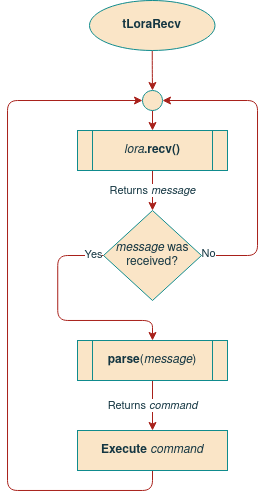
\includegraphics[width=.5\textwidth]{09sw_specification/Gateway/cgateway/tlorarecv}
	\caption{Flowchart: CGateway tLoraRecv method.}
	\label{fig:gwtLoraRecv}
\end{figure}

\clearpage
This task, presented in figure \ref{fig:gwtTCPRecv}, is responsible for receiving the messages sent by the remote system to the local systems. Unlike the \textit{tsend} tasks, this thread never enters the sleep state because one can receive a message at any moment. If it is received a message, then one can push the message to the messages queue in CLoraComm, signaling its thread to send the message, via LoRa communication.

\begin{figure}[H]
	\centering
	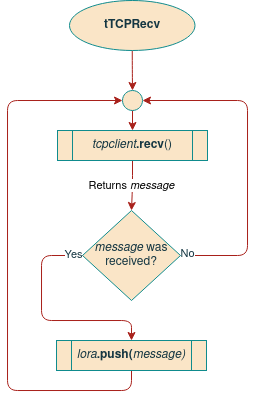
\includegraphics[width=.5\textwidth]{09sw_specification/Gateway/cgateway/ttcprecv}
	\caption{Flowchart: CGateway tTCPRecv method.}
	\label{fig:gwtTCPRecv}
\end{figure}

%*****************************
\clearpage
\myparagraph{CTCPclient Methods}

A TCPclient can be created through the use of the constructor, shown in figure \ref{fig:TCPclientconstructor}. This connects to a given server, defined by the string \textit{host}, and to the port \textit{port}, via TCP-IP and initializes all the private members.

\begin{figure}[H]
	\centering
	\includegraphics[width=.36\textwidth]{09sw_specification/Gateway/ctcpclient/constructor}
	\caption{Class Diagram: CTCPclient constructor.}
	\label{fig:TCPclientconstructor}
\end{figure}

As in CLoraComm, this class must implement \textit{recvFunc} and \textit{sendFunc}, as they are pure virtual methods from CCommunication. 

In this class, one will use existent functions \textit{TCPReceive} and \textit{TCPSend} to implement TCP-IP communication, as shown in figures \ref{fig:TCPclientrecvfunc} and \ref{fig:TCPclientsendfunc}. This functions make use of socket associated with the TCP-IP established connection.

\begin{figure}[H]
	\centering
	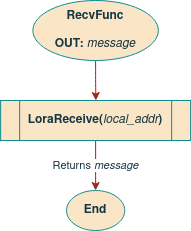
\includegraphics[width=.35\textwidth]{09sw_specification/Gateway/ctcpclient/recvfunc}
	\caption{Flowchart: CTCPclient recvFunc method.}
	\label{fig:TCPclientrecvfunc}
\end{figure}

\begin{figure}[H]
	\centering
	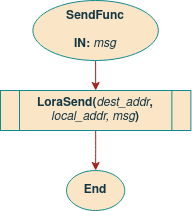
\includegraphics[width=.35\textwidth]{09sw_specification/Gateway/ctcpclient/sendfunc}
	\caption{Flowchart: CTCPclient sendFunc method.}
	\label{fig:TCPclientsendfunc}
\end{figure}

%**********************************************************
\clearpage
\section{Remote System}
%**********************************************************
The remote system is responsible for the communication between the local systems and the internet. In this project, the internet is used to maintain a cloud database, so the remote system does the data bridge between the network of street lampposts and a cloud. As one can see in figure \ref{fig:rs_overview}, the remote system is composed by the main process and a daemon process \textit{dServerSend}. The main process may be composed of a server and varoius clients, being the messages from each client received and processed in this process. The messages are sent to the clients in the daemon process \textit{dServerSend}. The communication between the two processes is done using message queues, so when a command is received and successfully parsed, the main process sends the command output to the daemon using the message queue.

\begin{figure}[H]
	\centering
	\includegraphics[width=.6\textwidth]{09sw_specification/RS/overview}
	\caption{Inter-process Communication between Main Process and Daemon.}
	\label{fig:rs_overview}
\end{figure}

%**********************************************************
\subsection{Class Diagram}
In figure \ref{fig:rs_classDiag} is represented the class diagram of the remote system. The class \textit{CTCPServer} is the main class of the system, that initializes the objects of each class, listed below. 

\begin{itemize}
	\item \textbf{CTCPServer:} main class, responsible for creating the server, the client objects, each time a client connects to the server and for sending the messages to the clients;
	\item \textbf{CClient:} client class, stores the clients information and receives their messages;
	\item \textbf{CDataBase:} provides an interface between the server and the database.

\end{itemize}

\begin{figure}[H]
	\centering
	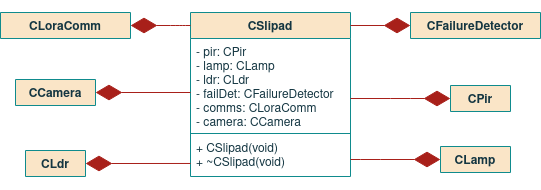
\includegraphics[width=.9\textwidth]{09sw_specification/RS/ClassDiagram}
	\caption{Remote System Class Diagram.}
	\label{fig:rs_classDiag}
\end{figure}

%****************************
\myparagraph{Class CTCPServer}

This class is responsible for creating the server, using \textit{createServer} function, allowing multiple clients to connect and send them messages, with the thread \textit{tSend}. When a client connects to the server, this class creates a new instance of the class \textit{CClient}. Each client can be of a different type of device like website, mobile application or gateway. The clients are assigned to their respective list of clients that are \textit{webSList}, \textit{appList} and \textit{gatewayList}, respectively. To do the interface with the database, this class also has an instance of the class database. In figure \ref{fig:CTCPServer}, one can see the class \textit{CTCPServer} diagram.

\begin{figure}[H]
	\centering
	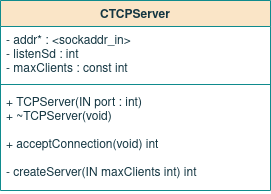
\includegraphics[width=.6\textwidth]{09sw_specification/RS/CTCPServer/CTCPServer}
	\caption{Class Diagram: CTCPServer.}
	\label{fig:CTCPServer}
\end{figure}

%****************************
\myparagraph{Class CClient}

The class \textit{CClient}, represented in figure \ref{fig:CClient}, is responsible for storing information about a client connected to the server, like the \textit{cmdList}, a vector that stores all the client commands list and \textit{clientSock}, and also for receiving messages from the clients in the thread \textit{tRecv}. The \textit{clientSock} has information about the client connected such as its \textit{state}, its client identification (\textit{index}), its name in \textit{clientName}, its file descriptor \textit{sockFd} and its type of client \textit{type}, that can be: \textit{GATEWAY}; \textit{WEBSITE}; or \textit{APPLICATION}.

\begin{figure}[H]
	\centering
	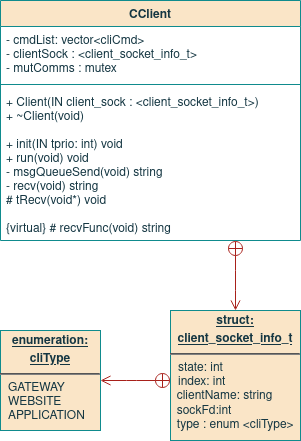
\includegraphics[width=.6\textwidth]{09sw_specification/RS/CClient/CClient}
	\caption{Class Diagram: CClient.}
	\label{fig:CClient}
\end{figure}

%****************************
\myparagraph{Class CDataBase}

This class diagram is shown in figure \ref{fig:CDataBase}, and is responsible for implement the interface between the server and the database, having for that a pointer to a database of type \textit{MYSQL}. To interact with the database, the server must first prepare a query, using the function \textit{prepareQuery}, and can update or get data from the database, using the prepared query and the functions \textit{updateData} and \textit{getData}, respectively.

\begin{figure}[H]
	\centering
	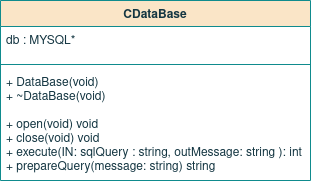
\includegraphics[width=.5\textwidth]{09sw_specification/RS/CDataBase}
	\caption{Class Diagram: CDataBase.}
	\label{fig:CDataBase}
\end{figure}

%**********************************************************
\subsection{Task Overview}
One can define and describe briefly how the remote system is implemented, making use of threads and processes. 

\begin{itemize}
	\item \textbf{tSend:} sends a message to a client;
	\item \textbf{tRecv:} receives a message from the clients.
\end{itemize}

%**********************************************************
\subsection{Task Priority}
As the two threads \textit{tRecv} and \textit{tSend} run in two different processes, daemon process and main process, respectively, one needs to define the threads priority assignment for the two processes. The priority assignment diagram for the remote system main process is represented in figure \ref{fig:rsMainPrio} and for the daemon process is shown in the figure \ref{fig:rsDaemonPrio}. 

\begin{figure}[H]
	\centering
	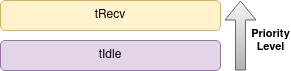
\includegraphics[width=.5\textwidth]{09sw_specification/RS/MainPrio}
	\caption{Remote System Main Process Priority Assignment.}
	\label{fig:rsMainPrio}
\end{figure}

\begin{figure}[H]
	\centering
	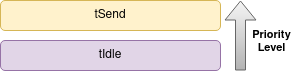
\includegraphics[width=.5\textwidth]{09sw_specification/RS/DaemonPrio}
	\caption{Remote System Daemon Process Priority Assignment.}
	\label{fig:rsDaemonPrio}
\end{figure}

%**********************************************************
\subsection{Task Synchronization}
As seen before, to have coordinate access to shared ressouces and services and avoid race conditions, the kernel has resources that provide synchronization between the tasks. 

\myparagraph{Mutexes}

The mutexes used for the remote system are listed bellow.

\begin{itemize}
	\item \textbf{CTCPServer::mutComms:} mutex used to protect the messages sending;
	\item \textbf{CClient::mutComms:} mutex used to protect the messages receiving.
\end{itemize}

\subsection{Task Communication}
\myparagraph{Message Queues}

In order to the main process communicate with the daemon process and send messages to the clients, one can use a message queue, named \textit{msgqComms}, that send the messages from the main process to the daemon process, containing the messages to be sent from the server to the clients.

%**********************************************************
\subsection{Flowcharts}
\myparagraph{CTCPServer}

In figure \ref{fig:ServerConst} is represented the constructor of the \textit{CTPCServer} class, that is responsible for creating the class variables, initializing the mutex and for creating the thread \textit{tSend} and the server socket in the port passed by argument.

\begin{figure}[H]
	\centering
	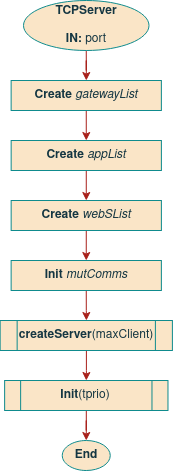
\includegraphics[width=.26\textwidth]{09sw_specification/RS/CTCPServer/ServerConst}
	\caption{Flowchart: CTCPServer Constructor.}
	\label{fig:ServerConst}
\end{figure}

The function that creates a server socket for a maximum number of clients, \textit{maxClient}, is represented in figure \ref{fig:RSCreateServer}. This function initiates a server socket with the IPv4 protocol connection.

\begin{figure}[H]
	\centering
	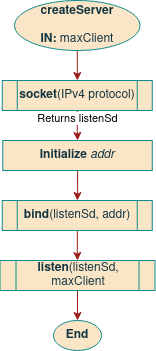
\includegraphics[width=.3\textwidth]{09sw_specification/RS/CTCPServer/CreateServer}
	\caption{Flowchart: CTCPServer createServer.}
	\label{fig:RSCreateServer}
\end{figure}

In figure \ref{fig:RSInit}, is shown the method that creates the thread \textit{tSend} with the priority \textit{tprio} passed by argument.

\begin{figure}[H]
	\centering
	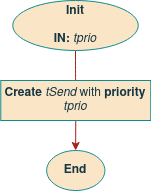
\includegraphics[width=.26\textwidth]{09sw_specification/RS/CTCPServer/Init}
	\caption{Flowchart: CTCPServer Init.}
	\label{fig:RSInit}
\end{figure}

The function \textit{run} is responsible for waiting for the termination of the thread \textit{tSend}.

\begin{figure}[H]
	\centering
	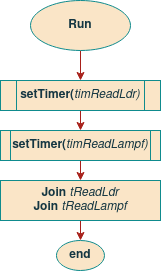
\includegraphics[width=.26\textwidth]{09sw_specification/RS/CTCPServer/run}
	\caption{Flowchart: CTCPServer run.}
	\label{fig:RSrun}
\end{figure}

In figure \ref{fig:RSsend} is represented the thread \textit{tSend}, which is responsible for sending a message to a client. It reads the messages to be sent in a message queue and send them to the recipient client.

\begin{figure}[H]
	\centering
	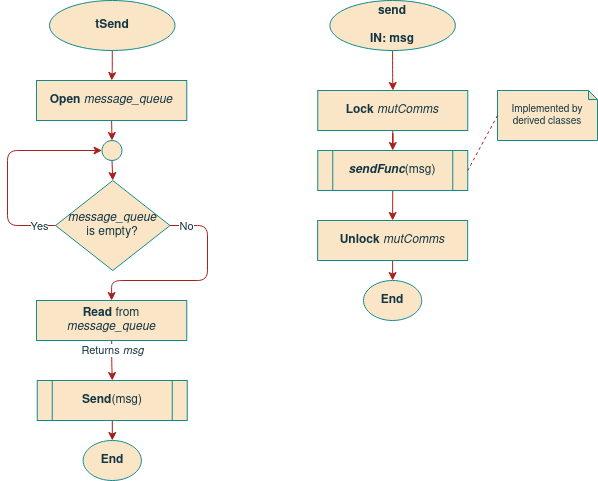
\includegraphics[width=.95\textwidth]{09sw_specification/RS/CTCPServer/send}
	\caption{Flowchart: CTCPServer tSend.}
	\label{fig:RSsend}
\end{figure}

%**********************************
\myparagraph{CClient}

In figure \ref{fig:ClientConst} is represented the constructor of the \textit{CClient} class. Every time a client connects to the server, it creates an instance of this class, passing by argument, the information about the client to initialize the \textit{clientSock} variable. The constructor also creates the command list that the type of client can execute, \textit{cmdList}, and the thread \textit{tRecv}.

\begin{figure}[H]
	\centering
	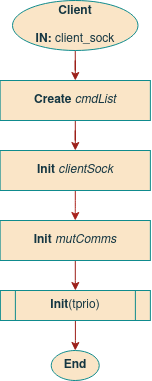
\includegraphics[width=.20\textwidth]{09sw_specification/RS/CClient/ConsClient}
	\caption{Flowchart: CClient Constructor.}
	\label{fig:ClientConst}
\end{figure}

The command list, \textit{cmdList} varies with the type of client:

\begin{itemize}
	\item \textbf{Mobile Application:} 
		\begin{itemize}
			\item Get;
			\item Update;
			\item Delete.
		\end{itemize}
	
	\item \textbf{Web Site:}
		\begin{itemize}
			\item Get.			
		\end{itemize}
	
	\item \textbf{Gateway:}
		\begin{itemize}
			\item Get;
			\item Update;
		\end{itemize}

\end{itemize}


%**********************************************************
\subsection{Start-up Process}

%**********************************************************
\subsection{Shutdown Process}


%**********************************************************
\clearpage
\section{Database}

\myparagraph{Relational Model}
The database's relational model is presented below.

\textbf{lamppost} (\underline{pole\_id}, \dashuline{gps}, pole\_status);

\textbf{location} (\underline{gps}, \dashuline{post\_code}, street\_name);

\textbf{region} (\underline{post\_code}, \dashuline{operator\_id}, parish, county, district);

\textbf{operator} (\underline{operator\_id}, operator\_name);

\textbf{parking\_space} (\underline{park\_id}, \dashuline{gps}, park\_type, park\_status).

\myparagraph{Logical Data Model}
The database's logical data model is presented in figure \ref{fig:database_er}.

\begin{figure}[H]
	\centering	
	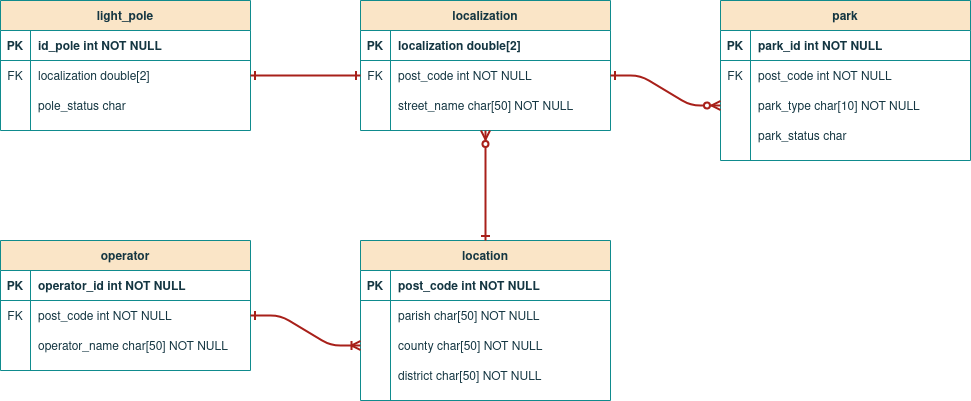
\includegraphics[width=1\textwidth]{09sw_specification/DataBase}
	\caption{Database Logical Data Model.}
	\label{fig:database_er}
\end{figure}

\myparagraph{Methods used}
Through the remote server, each remote client can have different permissions of access to the database, using the methods shown below.

\begin{itemize}
	\item \textbf{Mobile Application:} Add, Get, Update, Delete;
	\item \textbf{Web Site:} Get;
	\item \textbf{Gateway:} Update.	
\end{itemize}

%**********************************************************
\clearpage
\section{\ac{gui} Layouts}
In this section it is presented the \ac{gui} layouts, where the users can interact with the system.

\myparagraph{Mobile Application}

The mobile application is used by the operator, in order to manage the network of lampposts that is assigned to him. 

The first step is to login the system, so he has to insert is credentials \textit{ID Operator} and \textit{Password}, provided by the company. The login layout is shown in figure \ref{fig:login}. If the login was successful, then the operator can select one of this operations: \textit{Add New Lamppost}, \textit{Modify Lamppost} or \textit{Consult Lamppost Network}, as shown in figure \ref{fig:selectOperation}. The operator can also logout of his account.
%\begin{figure}[H]
%	\centering	
%	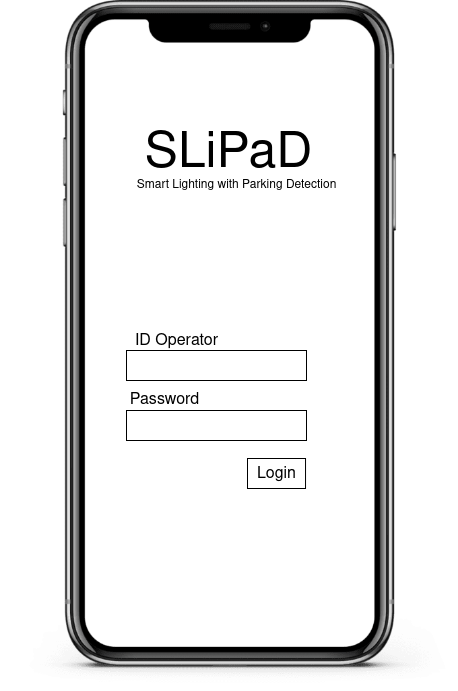
\includegraphics[width=.3\textwidth]{10gui_layouts/App/login}
%	\caption{Mobile Application Layout: Login.}
%	\label{fig:login}
%\end{figure}


%\begin{figure}[H]
%	\centering	
%	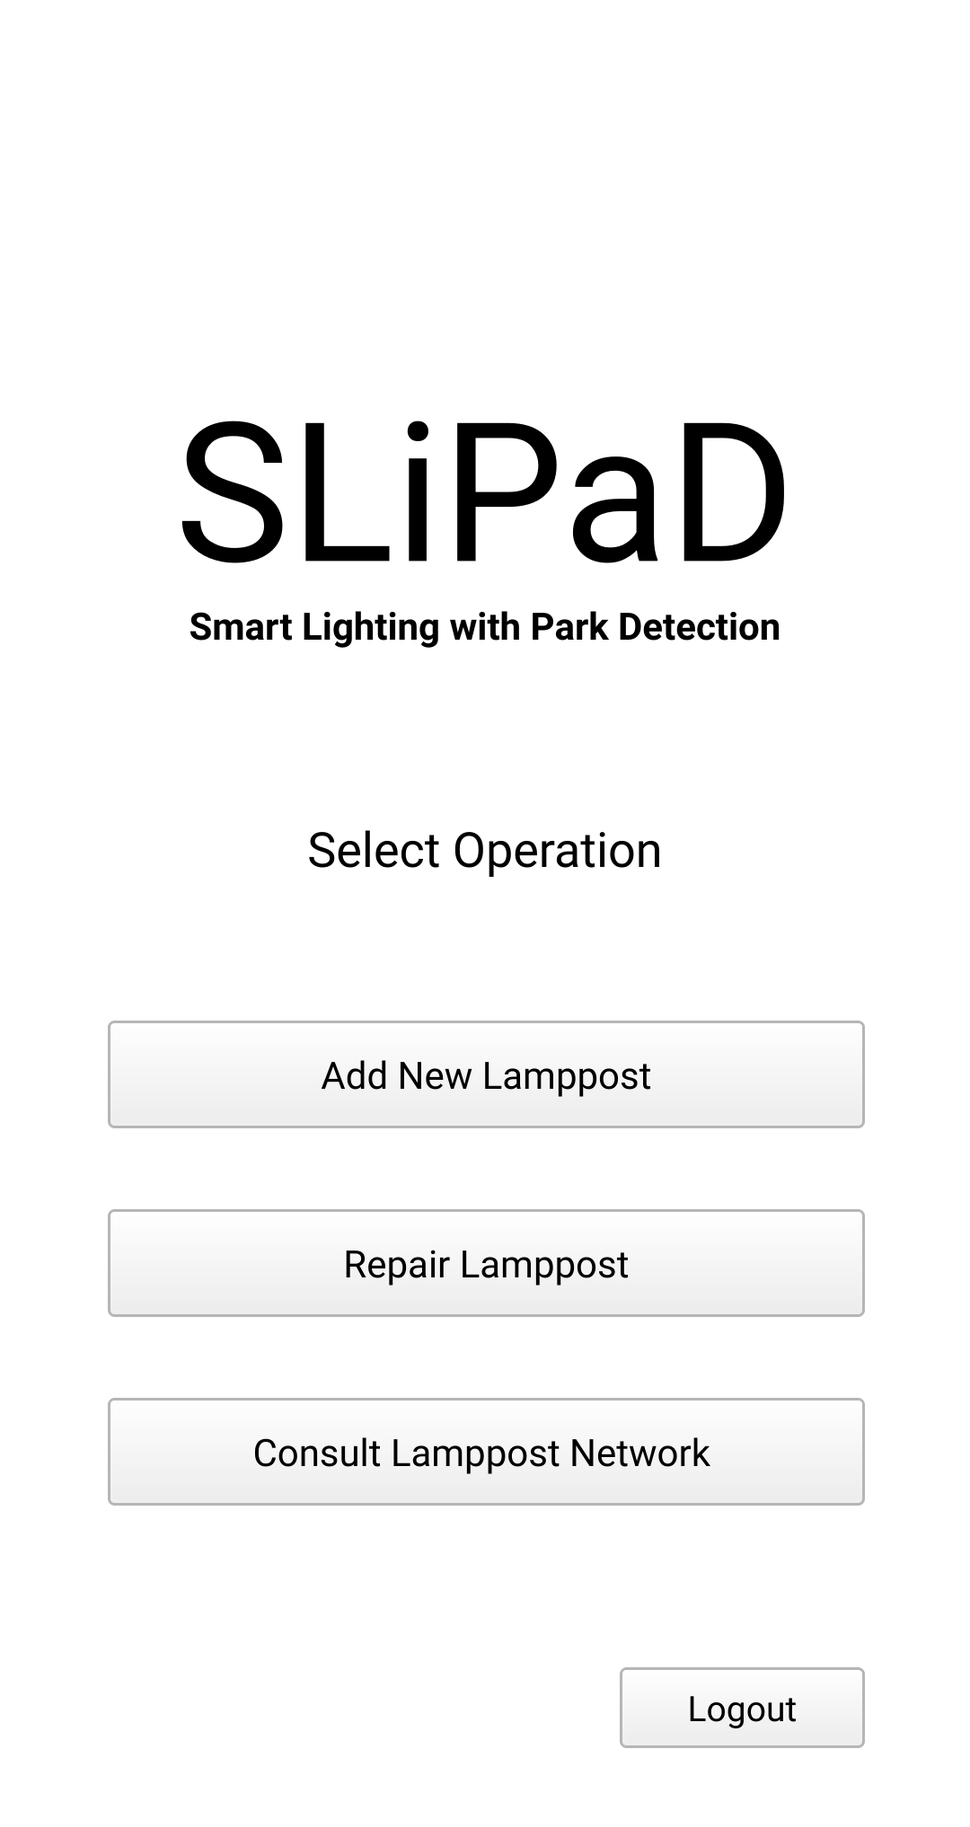
\includegraphics[width=.3\textwidth]{10gui_layouts/App/selectOperation}
%	\caption{Mobile Application Layout: Select Operation.}
%	\label{fig:selectOperation}
%\end{figure}

\begin{figure}[H]
	\centering
	\begin{subfigure}{.5\textwidth}
		\centering
		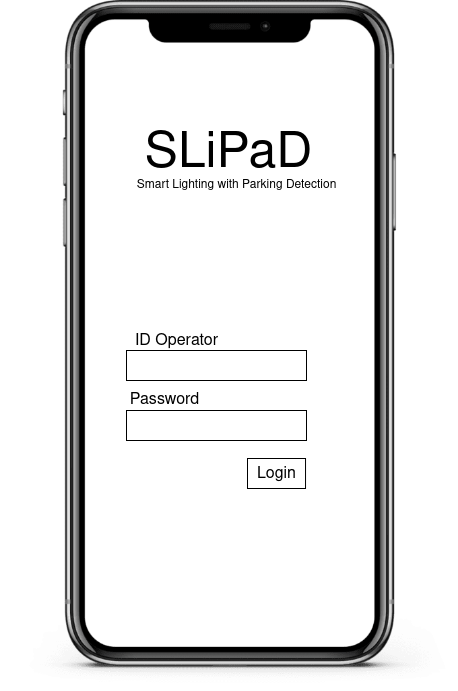
\includegraphics[width=.95\linewidth]{10gui_layouts/App/login}
		\caption{Login.}
		\label{fig:login}
	\end{subfigure}%
	\begin{subfigure}{.5\textwidth}
		\centering
		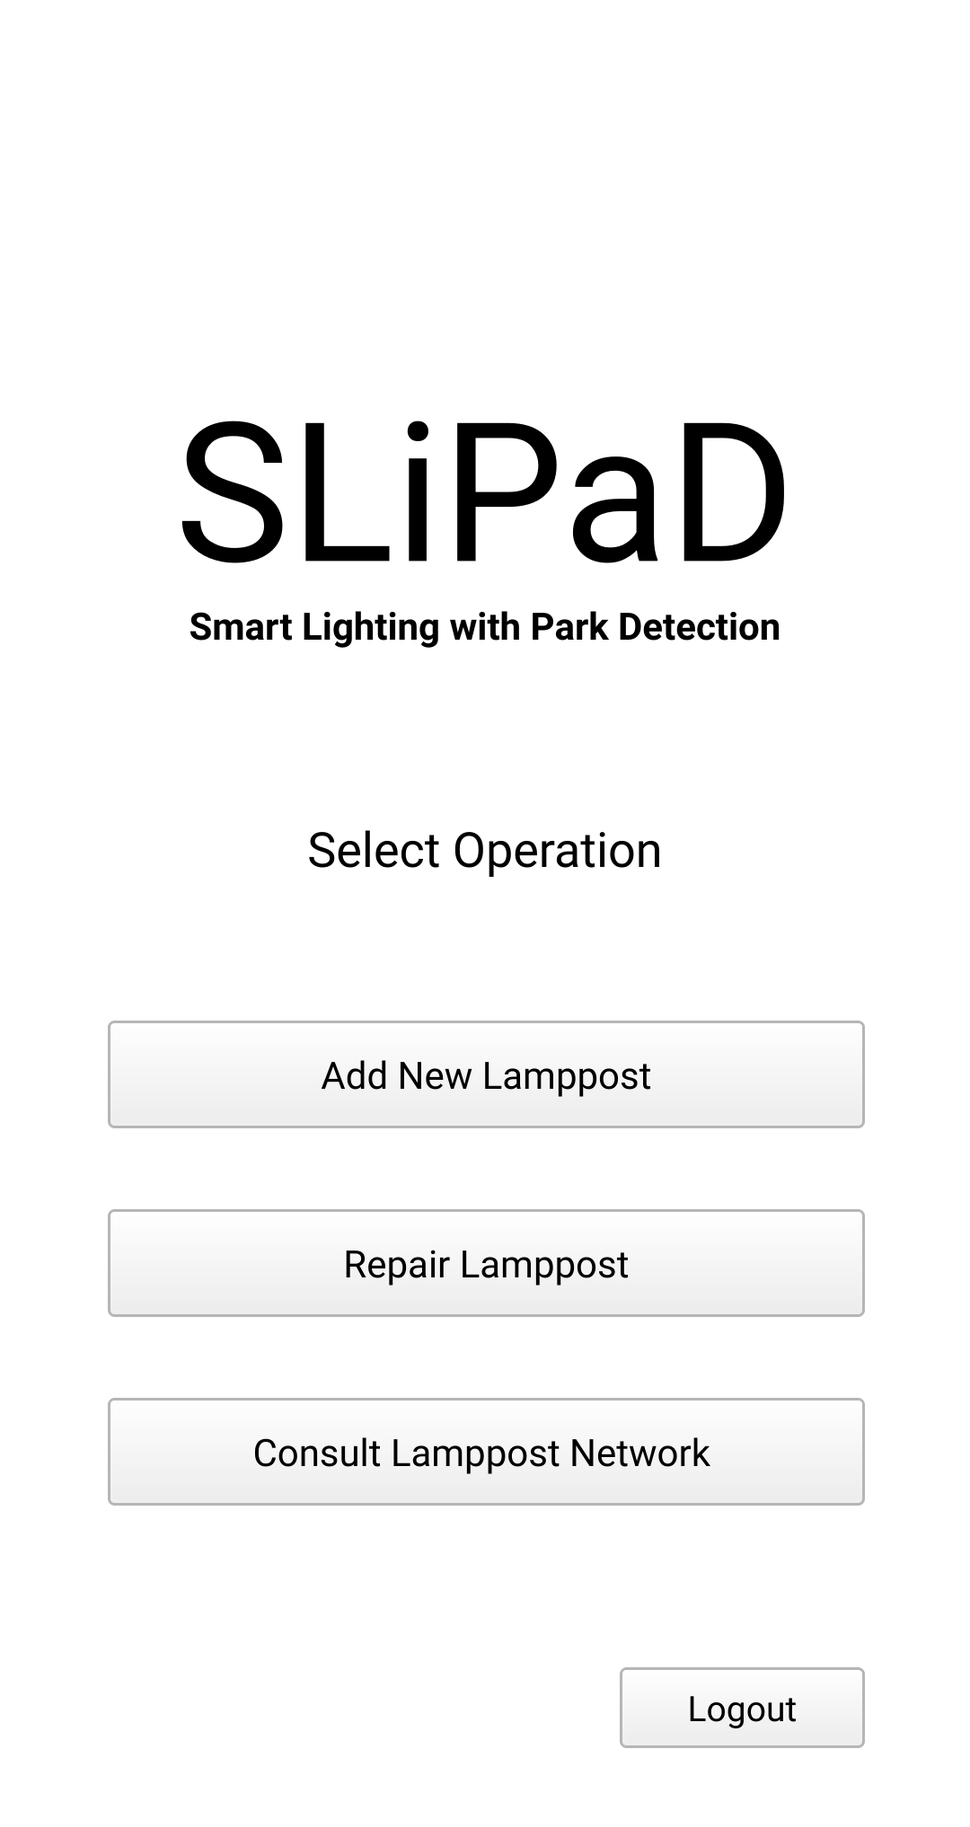
\includegraphics[width=.95\linewidth]{10gui_layouts/App/selectOperation}
		\caption{Select Operation.}
		\label{fig:selectOperation}
	\end{subfigure}
	\caption{Mobile Application Layout.}
	\label{fig:App}
\end{figure}

If the operator clicks on the \textit{Add New Lamppost} option, then he is redirected to the layout represented in figure \ref{fig:addNewLamppost}, where he can add a new lamppost to the network, inserting all the information about the location of the post or use his mobile device actual location. 

\begin{figure}[H]
	\centering	
	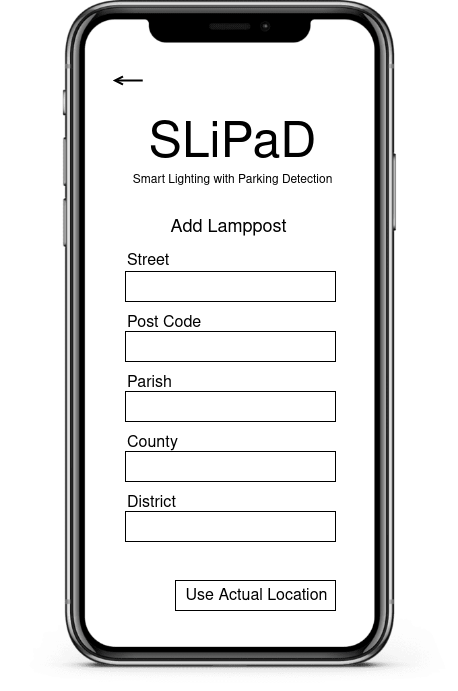
\includegraphics[width=.5\textwidth]{10gui_layouts/App/addNewLamppost}
	\caption{Mobile Application Layout: Add New Lamppost.}
	\label{fig:addNewLamppost}
\end{figure}

\clearpage
If the option chosen was the \textit{Modify Lamppost}, in order to change the lamppost status, he can insert the location of the post or use his mobile device actual location, as seen in figure \ref{fig:modifyLamppost}.

%\begin{figure}[H]
%	\centering	
%	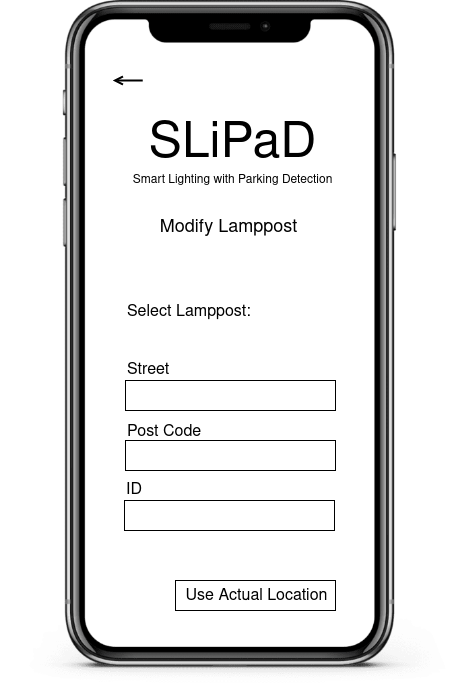
\includegraphics[width=.3\textwidth]{10gui_layouts/App/modifyLamppost}
%	\caption{Mobile Application Layout: Modify Lamppost.}
%	\label{fig:modifyLamppost}
%\end{figure}

If the lamppost selection was valid, then the layout represented in figure \ref{fig:acceptModify} appears, to the operator confirm that he wants to update the lamppost status.

%\begin{figure}[H]
%	\centering	
%	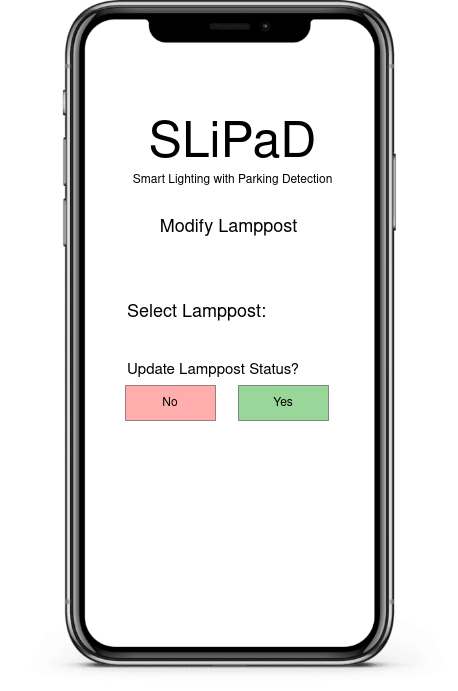
\includegraphics[width=.3\textwidth]{10gui_layouts/App/acceptModify}
%	\caption{Mobile Application Layout: Modify Lamppost Confirmation.}
%	\label{fig:acceptModify}
%\end{figure}

\begin{figure}[H]
	\centering
	\begin{subfigure}{.5\textwidth}
		\centering
		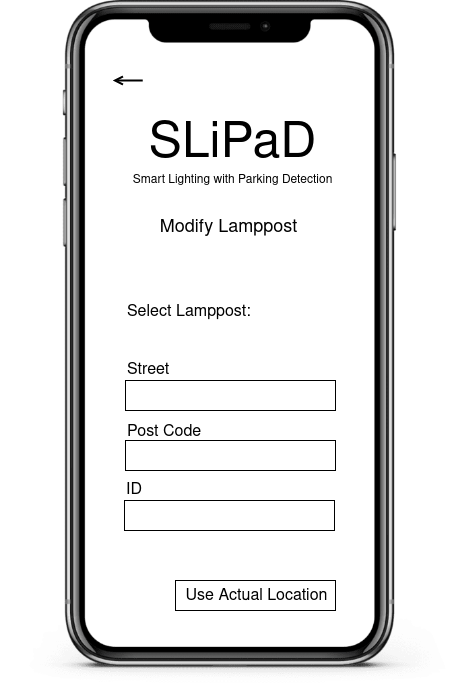
\includegraphics[width=.95\linewidth]{10gui_layouts/App/modifyLamppost}
		\caption{Modify Lamppost.}
		\label{fig:modifyLamppost}
	\end{subfigure}%
	\begin{subfigure}{.5\textwidth}
		\centering
		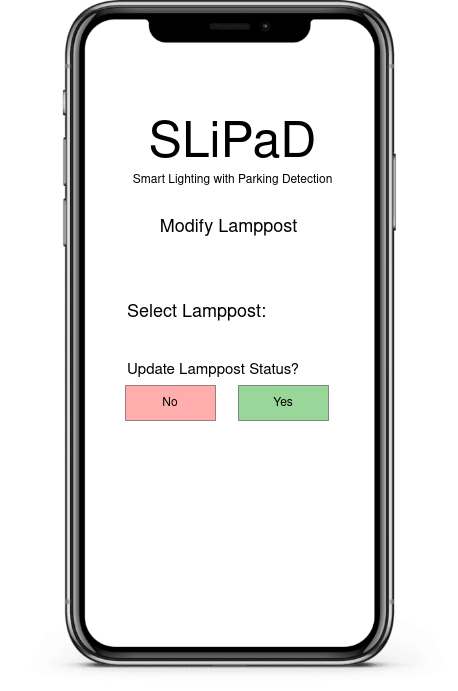
\includegraphics[width=.95\linewidth]{10gui_layouts/App/acceptModify}
		\caption{Modify Lamppost Confirmation.}
		\label{fig:acceptModify}
	\end{subfigure}
	\caption{Mobile Application Layout.}
	\label{fig:App2}
\end{figure}

\clearpage
On the other hand, if the operator selects the option \textit{Consult Lamppost Network}, the network information will appear like shown in figure \ref{fig:consultNetwork}, where the red point are lampposts with a broken lamp and the green points are the lampposts with no lamp problems.

\begin{figure}[H]
	\centering	
	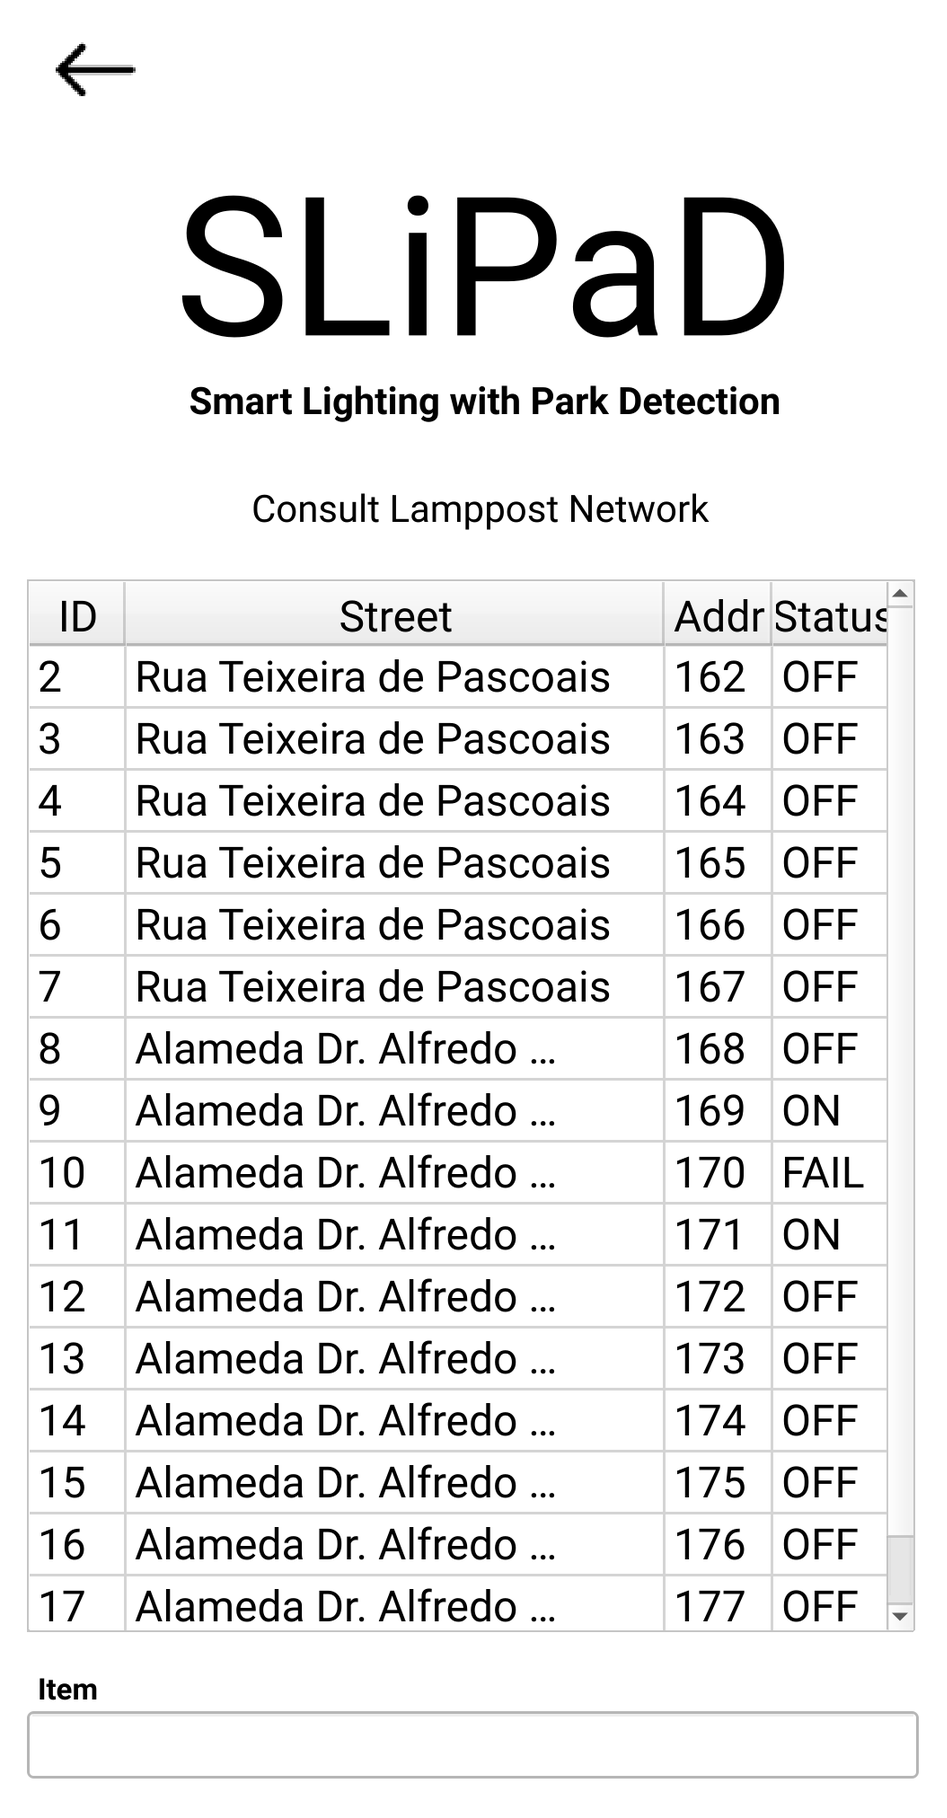
\includegraphics[width=.5\textwidth]{10gui_layouts/App/consultNetwork}
	\caption{Mobile Application Layout: Consult Lamppost Network.}
	\label{fig:consultNetwork}
\end{figure}

\clearpage
\myparagraph{Web Site}

The Web Site can be used by a user that wants to know where there are parking spots available near a location. 

When the user enters the site, it is presented a menu where he can insert the location where he wants to know the parking spots availability or use his actual location, as seen in figure \ref{fig:enterLocation}.

%\begin{figure}[H]
%	\centering	
%	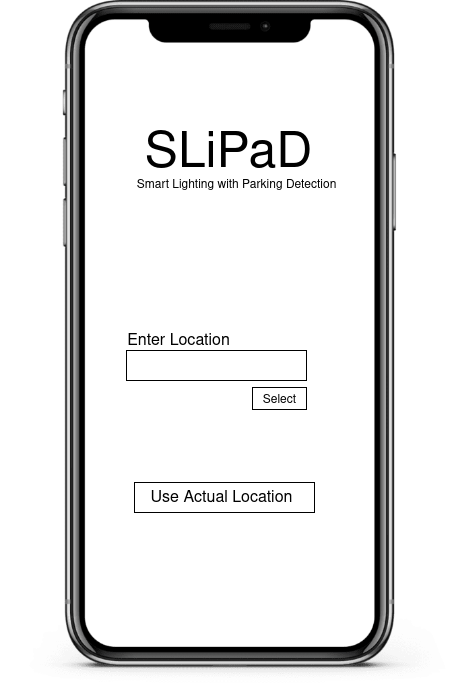
\includegraphics[width=.3\textwidth]{10gui_layouts/WebSite/enterLocation}
%	\caption{Web Site Layout: Enter Location.}
%	\label{fig:enterLocation}
%\end{figure}

After inserting the location, it will be shown the parking spots available near the location inserted, as seen in figure \ref{fig:parksEmpty}, where the red points represent the location of an empty parking spot.

%\begin{figure}[H]
%	\centering	
%	\includegraphics[width=.3\textwidth]{10gui_layouts/WebSite/parksEmpty}
%	\caption{Web Site Layout: Empty Parking Spots Location.}
%	\label{fig:parksEmpty}
%\end{figure}

\begin{figure}[H]
	\centering
	\begin{subfigure}{.5\textwidth}
		\centering
		\includegraphics[width=\linewidth]{10gui_layouts/WebSite/enterLocation}
		\caption{Enter Location.}
		\label{fig:enterLocation}
	\end{subfigure}%
	\begin{subfigure}{.5\textwidth}
		\centering
		\includegraphics[width=\linewidth]{10gui_layouts/WebSite/parksEmpty}
		\caption{Empty Parking Spots Location.}
		\label{fig:parksEmpty}
	\end{subfigure}
	\caption{Web Site Layout.}
	\label{fig:webSite}
\end{figure}


%**********************************************************
% TOOLS, COTS and THIRD PARTY LIBRARIES
\section{Tools}

\begin{itemize}
	\item \textbf{Buildroot:} Tool to configure and generate the Raspberry Pi Kernel image;
	\item \textbf{C/C++:} Programming language used to develop local system and remote system core;
	\item \textbf{Qt Creator:} Cross-platform IDE used for the Mobile Application development;
	\item \textbf{HTML:} Programming language chosen for the WebSite development;
	\item \textbf{Python:} Programming language chosen for the Haar cascade training stage;
	\item \textbf{MySQL:} Relational database management system used for the remote server database;
%	\item \textbf{MQTT:}
\end{itemize}

\section{COTS}

\begin{itemize}
	\item \textbf{POSIX Threads API:} Used for thread creation and management;
	\item \textbf{OpenCV API:} Used for image capture and processing;
	\item \textbf{Qt API:} Used for the GUI;
	\item \textbf{RaspiCam API:} C++ API for using Raspberry camera with/without OpenCv;
	\item \textbf{Cloudant API:} IBM cloud service that executes transactions in databases; ???
	\item \textbf{Google Cloud SQL:} Google Cloud service that allows for immutable data storage and retrieval;
\end{itemize}

\section{Third-Party Libraries}

\begin{itemize}
	\item \textbf{Light Sensor (TSL258x) Device Driver:} Open-source device driver used for interfacing with the luminosity sensor \cite{code_tsl};
	\item \textbf{LoRa SX1278 Library:} An Arduino open-source library for sending and receiving data using LoRa radios \cite{sx1278_lib}. This is implemented to the Arduino board, but it will be adapted to the Raspberry Pi 4 Model B.
\end{itemize}

